\documentclass{article}

\usepackage[english]{babel}

\usepackage[letterpaper,top=2cm,bottom=2cm,left=3cm,right=3cm,marginparwidth=1.75cm]{geometry}

\usepackage{amsmath}
\usepackage{graphicx}
\usepackage{tikz}
\usetikzlibrary{arrows}
\usetikzlibrary{arrows.meta,bending,chains}
\newcommand{\diff}{\mathop{}\!\mathrm{d}}
\usepackage[colorlinks=true, allcolors=blue]{hyperref}
\usepackage{imakeidx}
\makeindex[columns=3, title=Alphabetical Index, intoc]

\title{Progetto e PMBOK}
\author{Lorenzo Sanseverino 5DSA}

\begin{document}
\maketitle



\tableofcontents
\section{Definizione Di Progetto}

In ambito lavorativo ed aziendale un progetto è uno sforzo \textcolor{red}{temporaneo} intrapreso con lo scopo di crearea un \textcolor{red}{prodotto/servizio} unico e di qualità. \index{section}

\subsection{Elemetti di un progetto e triangolo dal triplice vincolo}
In un progetto è solito trovare quattro elemetti in comune, su cui si baserà tutto lo sviluppo dello stesso, essi sono:

\begin{itemize}
\item Obiettivo
\item Scadenza
\item Unicità
\item Personale ed impiego delle risorse umane
\end{itemize}

In oltre, è solito fare riferimento al triangolo dal triplice vincolo.
\begin{figure}[h]
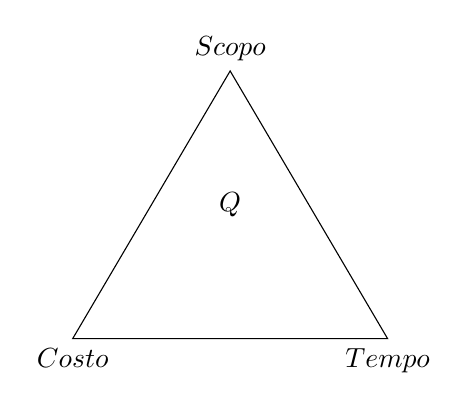
\begin{tikzpicture}
    \draw (0,0) node[anchor=north]{$Costo$}
        -- (4,0) node[anchor=north]{$Tempo$}
        -- (2,3.4) node[anchor=south]{$Scopo$}
        -- cycle    
        (2, 1.7) node[anchor=center]{$Q$};
\end{tikzpicture}
\caption{Triangolo dal triplice vincolo}
\label{t}
\end{figure}
Come è possibile visualizzare, nel caso in cui si dovesse dare più importanza ad uno di questi vincoli il triangolo non sarebbe più equilatero e bisognerebbe andare ad investire/magari perdere tempo per ri-aggiustarlo.
Molte volte è possibile trovare al centro una Q di Quality, questo fa riferimento ad una politica aziendale del cliente soddisfatto, \textit{\textcolor{red}{Total Quality Management}}, ossia si da la massima attenzione alla qualità del prodotto e ad offrire servizi ai clienti.

\section{Definizione di PMBOK e Project Management}
Nell'ultimo decennio si è visto come il concetto di progetto si sia diffuso sempre di più nelle varie aziende, e ciò ha portato alla necessità di metologie per gestirlo.
I motivi della sua diffusione sono tanti e ben distinti, ma possono essere riassunti in tre punti:
\begin{itemize}
    \item \textbf{Attività su commessa}
    \item \textbf{Problemi una tantum}
    \item \textbf{Strumento di innovazione}
\end{itemize}
La gestione del progetto attualemte è una vera e propria disciplina che prende il nome di \textbf{Project Management}.
Come concetti base della disciplina si può parlare di \textbf{CPM} (Critical Path Method, ossia di lavorare nella peggiore delle ipotesi per essere pronti ad ogni evenienza), il \textbf{PERT} (Program Evalutation and Review Tecnique, ossia valutare tempo e costo in rapporto ai rischi) ed il diagramma di \textbf{Gantt} (Utile per la gestione del tempo tramite piccole scadenze prefissate).
Tutto ciò viene descritto e ben spiegato nel \textbf{Project Management Body of Knowledge} che consiste in una vera e propria guida manageriale che ha lo scopo di definire linee guida per la gestione ed elaborazione di un progetto.

\subsection{Aree di Gestione}
Per descrivere le linee guida della gestione del progetto il PMBOK fa riferimento a 10 aree di gestione da membri diversi del gruppo.
\begin{enumerate}
    \item Gestione dell'ambito
    \item Gestione dei tempi
    \item Gestione dei costi
    \item Gestione della qualità
    \item Gestione delle risorse umane
    \item Gestione della comunicazione
    \item Gestione del rischio
    \item Gestione delle forniture
    \item Gestione delle integrazione dei processi
\end{enumerate}

\section{Figure del Project Management}

Le figure di un progetto e ciò che gli stessi devono fare/pensare può essere schematizzato con questo schema:

\begin{figure}

\begin{center}
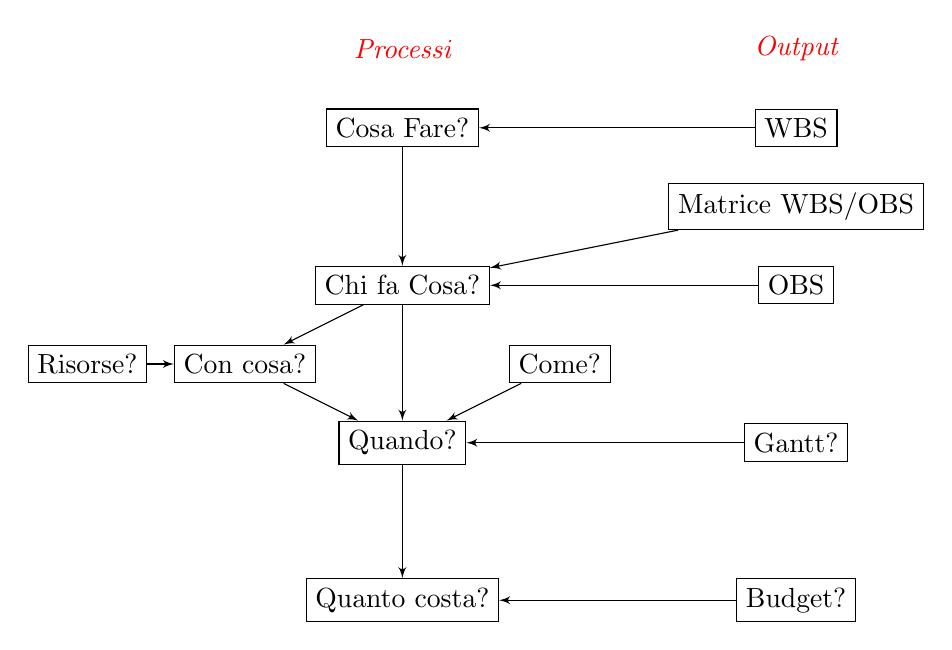
\begin{tikzpicture}
\node at (0, 1) {\textit{\textcolor{red}{Processi}}};
\node at (5, 1) {\textit{\textcolor{red}{Output}}};

\node[draw, rectangle] (s1) at (0,0) {Cosa Fare?};
\node[draw, rectangle] (t1) at (5,0) {WBS};

\node[draw,rectangle] (s2) at (0,-2) {Chi fa Cosa?};
\node[draw,rectangle] (t2) at (5,-2) {OBS};
\node[draw,rectangle] (t21) at (5,-1) {Matrice WBS/OBS};

\node[draw,rectangle] (s3) at (-2,-3) {Con cosa?};
\node[draw,rectangle] (t3) at (2,-3) {Come?};
\node[draw,rectangle] (t31) at (-4,-3) {Risorse?};


\node[draw,rectangle] (s4) at (0,-4) {Quando?};
\node[draw,rectangle] (t4) at (5,-4) {Gantt?};

\node[draw,rectangle] (s5) at (0,-6) {Quanto costa?};
\node[draw,rectangle] (t5) at (5,-6) {Budget?};
\path
    (t1) edge[->, >=latex', ] (s1)
    (s1) edge[->, >=latex', ] (s2)
    (t2) edge[->, >=latex', ] (s2)
    
    (s2) edge[->, >=latex', ] (s3)
    (s4) edge[->, >=latex']   (s5)
    (t31) edge[->, >=latex'] (s3)
    
    (t21) edge[->, >=latex',] (s2)
    (s3)  edge[->, >=latex'] (s4)
    (t3)  edge[->, >=latex'] (s4)
    (s2)  edge[->, >=latex'] (s4)
    (t4) edge[->, >=latex', ] (s4)
    (t5) edge[->, >=latex', ] (s5);
\end{tikzpicture}
\end{center}
\label{Schema}
\caption{Schema organizzativo}
\end{figure}

In una azienda, a gestire l'organizzazione e lo sviluppo di un progetto, è possibile trovare svariate figure che variano a seconda del tipo di azienda e progetto.
Una figura in comune per il Project Management è sicuramente quella del \textbf{Project Management}.
È la figura più importante, definito anche regista del progetto, lui non si preoccupa delle competenze tecniche ma di supervisione e coordinare tutti i membri del gruppo.
Si occupa di individuare la struttura di un progetto e di avviarla rispettando i vincoli (vedi Fig \ref{t}), deve organizzare un sistema di monitoraggio, una documentazione e cosa più importante prendere decisione sul \textbf{Make Or Buy}.


\section{Fasi di un Progetto}
Un progetto nasce da una idea/opportunità per arrivare ad un risultato, ponendosi degli obiettivi.
Ogni obiettivo è raggiungibile mediante sforzi coordinati da parte del gruppo di lavoro seguendo delle fasi.
Generalmente le fasi si dividono in 4:

\begin{enumerate}
\item Concezione
\item Definizione
\item Realizzazione
\item Chiusura	
\end{enumerate}

\end{document}